\NeedsTeXFormat{LaTeX2e}[2005/12/01]
%%    2009/03/12 v1.0 GAUBM Vorlage für Abschlussarbeiten Physik
%% Template fuer Bachelor- und Masterarbeiten
%% an der Fakultaet fuer Physik (c) Thomas Pruschke der GA Universität
%% Verbesserungsvorschlaege bitte an pruschke@theorie.physik.uni-goettingen.de
%%
%% Benoetigte Pakete: datenumber
%%


%% scrbook - Ersatz für LaTeX book Klasse aus dem KOMA Script
%% Moegliche Optionen: diejenigen der Klasse scrbook ausser titlepage

%% deutsche Arbeit:
\documentclass[bachelor,       %% Typ der Arbeit: bachelor oder master
               twoside,        %% zweiseitiges Layout
               BCOR10mm,       %% Bindekorrektur 10 mm
%               liststotoc,nomtotoc,bibtotoc, %% Aufnahme der div. Verzeichnisse
                                              %% ins Inhaltsverzeichnis
               english,ngerman, %% Alternativspr. Englisch, Dokumentspr. Deutsch
%               ngerman,english  %% Alternativspr. Deutsch, Dokumentspr. Englisch
%               final,          %% Endversion; draft fuer schnelles Kompilieren
%				draft,
               ]{GAUBM}

\usepackage{setspace}  %% Zur Setzung des Zeilenabstandes
\usepackage{babel}     %% Sprachen-Unterstuetzung
\usepackage{calc}      %% ermoeglicht Rechnen mit Laengen und Zaehlern
\usepackage[T1]{fontenc}       %% Unterstutzung von Umlauten etc.
%\usepackage[latin1]{inputenc}  %% 
%% in aktuellem Linux & MacOS X wird standardmaessig UTF8 kodiert!
\usepackage[utf8]{inputenc}    %% Wenn latin1 nicht geht ...

\usepackage{amsmath,amssymb} %% zusaetzliche Mathe-Symbole

\usepackage{lmodern} %% type1-taugliche CM-Schrift als Variante zur
                     %% "normalen" EC-Schrift
%% Paket fuer bibtex-Datenbanken
\usepackage[comma,super,sort&compress]{natbib}
\bibliographystyle{abbrvnat}

\newcommand{\tabheadfont}[1]{\textbf{#1}} %% Tabellenkopf in Fett
\usepackage{booktabs}                      %% Befehle fuer besseres Tabellenlayout
\usepackage{longtable}                     %% umbrechbare Tabellen
\usepackage{array}                         %% zusaetzliche Spaltenoptionen
\usepackage{siunitx}
\usepackage{verbatim}
% Mehrere Abbildungen nebeneinander
% Beispiel:
% \begin{figure}[htb]
%   \centering
%   \subfigure[<+Beschriftung 1+>\label{fig:<+label1+>}]
%   {\includegraphics[width=0.49\textwidth]{<+grafik1+>}}
%   \hfill
%   \subfigure[<+Beschriftung 2+>\label{fig:<+label2+>}]
%   {\includegraphics[width=0.49\textwidth]{<+grafik2+>}}
%   \caption{<+Beschriftung allgemein+>}
%   \label{fig:<+label-gesamt+>}
% \end{figure}
\usepackage{subfigure}

\usepackage{graphicx}
\graphicspath{{./Bilder/}}

\usepackage{adjustbox}
%Fußnoten zwingend auf diese Seite setzen
\interfootnotelinepenalty=1000

%keine Einrückung, wenn Latex doppelte Leerzeile
\parindent0pt

%% umfangreiche Pakete fuer Symbole wie \micro, \ohm, \degree, \celsius etc.
\usepackage{textcomp,gensymb}

%\usepackage{SIunits} %% Korrektes Setzen von Einheiten
\usepackage{units}   %% Variante fuer Einheiten

%% Hyperlinks im Dokument; muss als eines der letzten Pakete geladen werden
\usepackage[pdfstartview=FitH,      % Oeffnen mit fit width
            breaklinks=true,        % Umbrueche in Links, nur bei pdflatex default
            bookmarksopen=true,     % aufgeklappte Bookmarks
            bookmarksnumbered=true  % Kapitelnummerierung in bookmarks
            ]{hyperref}

%% Weiter benoetigte Pakete: datenumber
%% Falls dieses Paket nicht in der Installation vorhanden ist,
%% kann es von der Seite mit diesem Template heruntergeladen werden
%% und in einem LaTeX bekanntem Verzeichnis installiert werden (notfalls
%% dem Verzeichnis mit der Arbeit).
\begin{document}
%%
%%                   Ab hier muessen die Anpassungen geschehen
%%
%% Hier den eigenen Namen einsetzen
\ThesisAuthor{Michael Alexander}{Lohmann}
%% Hier den Geburtsort einsetzen
\PlaceOfBirth{Randburg (RSA)}
%% Titel Arbeit. Das erste Argument ist der deutsche, das zweite der
%% englische Titel.
\ThesisTitle{Multi-Photon-Photoemission an Gold-Nanospitzen mit sichtbarem und nah-infrarotem Licht}{Multiphoton-photoemission at gold nanotips with visible and near-infrared light}
%% Erst- und Zweitgutacher/in
%% Ist der/die Betreuer/in nicht identisch mit dem/r Erstgutachter/in,
%% muss diese/r als optionales Argument angegeben werden.
\FirstReferee[Dr.\ Reiner Bormann und Benjamin Schröder]{Prof.\ Dr.\ Claus Ropers}
\Institute{4. Physikalischen Institut}
\SecondReferee{Prof.\ Dr.\ Christian Jooß}
%% Beginn und Ende des Anfertigungszeitraumes
\ThesisBegin{1}{4}{2016}
\ThesisEnd{15}{7}{2016}
%% DO NOT TOUCH THESE LINES!!!!
\frontmatter
\maketitle
\cleardoublepage
%% Zusammenfassung. Falls nicht gewuenscht, bitte auskommentieren.
\begin{abstract}
Ziel der Arbeit ist die erstmalige Untersuchtung des nichtlinearen Photoeffektes aus Gold-Nanospitzen über einen großen Wellenlängenbereich.
Dafür wurde ein Optisch Parametrischer Verstärker (OPA) verwendet, der Laserlicht mit kontinuierlich durchstimmbarer Wellenlänge liefert.
Der Laser-Puls wurde dazu verwendet, mit Multi-Photon-Photoemission Elektronen aus der Oberfläche auszulösen.\newline
Es zeigt sich, dass die Nichtlinearität (entspricht der Anzahl an benötigten Photonen) im untersuchten Bereich nicht stufenförmig (wie im einfachsten Modell), sondern annähernd linear ist.


%% Optional: Stichwoerter. Wenn nicht gewuenscht, koennen die beiden
%% folgenden Zeilen geloescht werden
  \bigskip\par
  \textbf{Stichwörter:} lokalisierte Elektronenemission, Gold Nano-Spitze, multiphoton Photoemission
\end{abstract}
%% So laesst sich in die andere Sprache umschalten (Englisch bzw. Deutsch)
\begin{otherlanguage}{english}
\begin{abstract}
The aim of this work is to determine the work function of Au nanotips.
An optic parametric amplifier was used to continuously vary the laser wavelength.
The fs-Laserpulses exracted electrons with multiphoton photoemission.\\
The results do show a nearly linear growth in the examined region instead of a stepfunction (like the simplest model).
  \bigskip\par
  \textbf{Keywords:} localized electron emission, gold nano-tip, multiphoton photoemission
\end{abstract}
\end{otherlanguage}

%% Ende des Vorspanns
\cleardoublepage
%% Ab hier 1 1/2 facher Zeilenabstand (durch setspace-Paket)
\onehalfspacing
%% Erzeugt Inhaltsverzeichnis
\tableofcontents

%% Hier kann man seine Bezeichnungsweisen erklaeren. Falls nicht
%% benoetigt, bis einschliesslich \end{nomenclature} auskommentieren
\begin{nomenclature}
%% Fuer die Berechnung der Spaltenbreiten muss \usepackage{calc}
%% geladen sein!
\section*{Lateinische Buchstaben}
\noindent
\begin{longtable}[l]{p{0.2\textwidth}p{0.7\textwidth-6\tabcolsep}p{0.1\textwidth}}
  \tabheadfont{Variable}&\tabheadfont{Bedeutung}&\tabheadfont{Einheit}\\\midrule\endhead
  $U_\text{Tip}$ & Spannung zwischen Spitze und Extraktor & $\unit{V}$\\
  $U_\text{Sup}$ & Spannung zwischen Suppressor und Extraktor & $\unit{V}$\\
  $U_p$ & Ponderomotive Energie & $\unit{J}$\\
  $e$ & Elementarladung & $\unit{Q}$\\
  $m_e$ & Elektronenmasse & $\unit{kg}$\\
  $I$ & Intensität des Lasers & $\unit{Wm^{-2}}$
\end{longtable}
\section*{Griechische Buchstaben}
\begin{longtable}[l]{p{0.2\textwidth}p{0.7\textwidth-6\tabcolsep}p{0.1\textwidth}}
  \tabheadfont{Variable}&\tabheadfont{Bedeutung}&\tabheadfont{Einheit}\\\midrule\endhead
  $\lambda$ & Wellenlänge & $\unit{nm}$\\
  $\omega$ & Frequenz & $\unit{Hz}$\\
  $\gamma$  & Keldysh-Parameter & $\unit{}$\\
  $\Phi$ & Austrittsarbeit & $\unit{eV}$
\end{longtable}
\section*{Indizes}
\begin{longtable}[l]{p{0.2\textwidth}p{0.8\textwidth-4\tabcolsep}}
  \tabheadfont{Index}&\tabheadfont{Bedeutung}\\\midrule\endhead
  $e$ & Elektron\\
  Tip & Nano-Spitze\\
  Sup & Supressor
\end{longtable}
\section*{Abk"urzungen}
\begin{longtable}[l]{p{0.2\textwidth}p{0.8\textwidth-4\tabcolsep}}
  \tabheadfont{Abkürzung}&\tabheadfont{Bedeutung}\\\midrule\endhead
  2D & zweidimensional\\
  3D & dreidimensional\\
  OPA & Optisch Parametrischer Verstärker\\
  MCP & Micro Channel Plate\\
  SHG & Second Harmonic Generation\\
  TEM & Transmissions Elektronen Mikroskop\\
  UTEM & Ultrafast TEM\\
  ULEED & Ultrafast Low Energy Elektron Defraction\\
  ATP & Above Threshhold Photoemission
\end{longtable}
\end{nomenclature}
%% \listoftables und \listoffigures sollten nur bei genuegender Anzahl Tabellen verwendet werden
%\listoffigures
%\listoftables

\mainmatter   %% Anfang Hauptteil

\chapter{Einleitung}
Ein grundlegendes Verständnis der Materie ist ein essentielles Ziel der Forschung.
Daher wurden gerade seit den dreißiger Jahren des 19. Jahrhunderts immer ausgefeiltere Mikroskopietechniken entwickelt \cite{ruska_1931}.
Die höchsten räumlichen Auflösungen bieten hierbei noch immer Rastertunnelmikroskope (engl. \textit{scanning tunneling microscopy}, kurz STM) und Transmissionenelektronenmikroskope (\textit{transmission elektron microscope}, kurz TEM).
Deren Auflösungsvermögen, welches wichtig ist, um makroskopische Prozesse auch auf mikroskopischer Skala zu verstehen, liegt zwar auf atomarer Ebene ($\approx\SI{1}{\angstrom}$), jedoch ist die Zeitauflösung beider Methoden sehr begrenzt.
Gerade um dynamische Prozesse wie strukturelle Änderungen und Phasenübergänge zu untersuchen ist dies jedoch wichtig.
Um auch die temporale Auflösung zu erhalten, ist eine Elektronenquelle notwendig, welche räumlich kohärente kurze Elektronenpulse bereitstellt (z.B. \citet{gulde_ultrafast_2014}).

Eine Lösungsmöglichkeit besteht darin, Nanospitzen mit Femtosekunden-Laserpulsen zu beleuchten.
Die kleine Emissionsfläche, die durch Feldverstärkung und elektrostatische Felder auf den nanometrischen Apex begrenzbar ist, gewährleistet eine hohe räumliche Kohärenz der $e^-$-Pulse.
Dieser Ansatz wurde bisher schon erfolgreich in der ultraschnellen niedrigenergetischen Beugung von Elektronen (ULEED) und der ultraschnellen Transmissionselektronenmikroskopie (UTEM) verwendet (z.B. \citet{gulde_ultrafast_2014} und \citet{barwick_4d_2008}).
<+Dabei wird die hohe Zeitauflösung durch das Pump-Probe verfahren erreicht, bei dem das Experiment sehr häufig wiederholt wird und durch Aufnahmen zu unterschiedlichen Zeitpunkten ein Verlauf aufgenommen wird.
Ein Laserpuls regt beispielsweise einen Phasenübergang an.
Der Elektronenpuls trifft nun mit variabler Verzögerung auf die zu untersuchende Position.
Dies ist allerdings nur machbar bei reversiblen Prozessen.+>

Um ein Elektron zu emittieren kann entweder die Energie eines einzelnen Photons ausreichen, um die Austrittsarbeit zu überwinden, oder es muss Multiphotonemission stattfinden.
Dabei treffen $N$ Photonen annähernd gleichzeitig auf ein Elektron.
Die Wahrscheinlichkeit der Emission ist proportional zu $I^N$, wobei $I$ die Intensität des einfallenden Lichtes beschreibt.

Allerdings stellten dabei zahlreiche Publikationen (s. Tab. \ref{tab:komische_steigungen}) fest, dass bei der Intensität der emittierten Elektronen eine nicht erwartete Anzahl an benötigten Photonen benötigt wird.
So stellte man bei vielen Experimenten beispielsweise eine benötigte Anzahl von $4.4$ Photonen zur Auslösung fest.

In dieser Arbeit soll diese nichtlineare Photoemission einer systematischen Untersuchung über einen breiten Wellenlängenbereich erfolgen. Im genauen wird eine Gold-Nanospitze mit fs-Pulsen mit \SI{1.5}{\eV} bis \SI{2.7}{\eV} Photonenergie beleuchtet.

Um die Wellenlänge des Lasers verändern zu können wurde einen Optisch Parametrischen Verstärker (OPA) verwendet, mit dessen Hilfe sich die Wellenlänge des Lasers kontinuierlich von $250-\SI{20000}{\nano\meter}$ durchstimmen lässt (Ausgangsleistungen nach Hersteller in Abb. \ref{fig:orpheus_tuningcurve}).
Im Rahmen dieser Arbeit wurde der Bereich von 460 bis \SI{850}{\nm} untersucht.



\chapter{Grundlagen}
In diesem Kapitel werden die grundlegenden Begriffe und Formeln für diese Arbeit eingeführt, sowie die dahinterstehende Theorie erklärt.

\section{Austrittsarbeit}
Mit dem Begriff Austrittsarbeit wird die Energie, die ben\"otigt wird, um ein Elektron aus einem Atom oder Festk\"orper zu entfernen.
Sie ist material- und strukturspezifisch. 

F\"ur das in dieser Arbeit verwendete Gold sind in Tabelle \ref{tab:austrittsarbeit} einige Messwerte aufgef\"uhrt, welche mit verschiedensten Methoden ermittelt wurden.
Zu erkennen ist, dass sie von der jeweiligen Kristallfl\"ache abh\"angt.
Aber auch bei der gleichen Kristallebene finden sich Unterschiede in den Ergebnissen (z.B. gibt es zu der (1 1 1)-Ebene Messwerte von 5.3 bis \SI{5.5}{\eV})


\begin{table}[h!]
\centering
\begin{tabular}{|c|c|c|c|}
\hline 
Quelle und Jahr& Kristallfläche & Austrittsarbeit [\unit{eV}] & Methode \\ 
\hline\hline
\citet[1931]{fowler_1931} & ? 			& 4.9 				& th \\\hline
\citet[1932]{dubridge_further_1932} & ? 	& 4.81 			& ph \\\hline

\citet[1966]{sachtler_work_1966} & ? 	& \numrange{5.30}{5.45} & ph \\\hline

\citet[1974]{trasatti_operative_1974} & ? 	& 4.8 		& ec \\\hline
\citet[1982]{pescia_spin_1982} & (1 1 1) 	& 5.5 		& ph \\\hline
\citet[1986]{koetz_1986} & ? 				& $5.1\pm0.15$ 		& XPS \\\hline
\citet[1990]{lecoeur_1990}	& (1 1 1) 		& $5.30\pm0.05$ 	& ph \\
					& (3 1 1) 		& $5.16\pm0.07$ 	& Kontakt \\
					& (1 1 0) 		& $5.12\pm0.07$ 	& Kontakt \\
					& (2 1 0) 		& $4.96\pm0.07$ 	& Kontakt \\\hline
\citet[2004]{crc}		&(1 0 0) 			& 5.47 				& ph \\
 				&(1 1 0) 			& 5.37 				& ph \\
				&(1 1 1) 			& 5.31 				& ph \\\hline
\end{tabular} 
\caption{Auftragung verschiedener Austrittsarbeiten nach verschiedenen Publikationen. Abkürzungen Methoden: th = thermisch, ph = photoelektrisch, ec = elektrochemisch, XPS = Röntgen-Photoelektron-Spektroskopie, Kontakt = Kontaktpotential zu (1 1 1)-Facette}
\label{tab:austrittsarbeit}
\end{table}


\section{Mechanismen der Photoemission}
Photoemission (PE) beschreibt die Auslösung von Elektronen aus Materie durch Bestrahlung mit Licht.
Dabei muss die absorbierte Energie die Austrittsarbeit übersteigen.

PE lässt sich in mindestens fünf Bereiche unterteilen, welche sich in der eingestrahlten Intensität $I$ unterscheiden:
\begin{itemize}
	\item\textit{klassischer (linearer) Photoeffekt}
	Der klassische Photoeffekt nach \textsc{Einstein} \cite{einstein1905} besagt, dass Elektronen aus einem Festkörper nur dann ausgelöst werden, wenn ein einzelnes Photon genügend Energie $W_\text{Ph}$ besitzt, um die Auslösearbeit $\Phi$ zu leisten.
	Diese ist bedingt durch die unterschiedliche Ladung von Atomkern und Elektron, weshalb sich diese anziehen und Energie aufgewendet werden muss, um sie zu trennen.
	Die Bilanzgleichung lautet dann
	\begin{align*}
	W_\text{El}=W_\text{Ph}-\Phi\quad .
	\end{align*}
	Es muss also gelten $W_\text{Ph}\geq\Phi$, damit die kinetische Energie des Elektrons $W_\text{EL}$ positiv ist.
	Eine größere Photonenenergie bewirkt eine höhere Überschussenergie.
	Kann man diese messen, so kann man Rückschlüsse auf die Austrittsarbeit schließen und mit der <+PhotoElektron Spektroskopie+> eine Analyse der Inhaltsstoffe einer Probe machen
	Für typische Metalle gilt $\Phi\approx4\ldots\SI7\electronvolt$ was einer Wellenlänge von höchstens \SI{300}{\nm} entspricht \cite{crc}.
	
	\item \textit{Multi-Photon-Emission}
	Nach Einstein ist nur die Photonenenergie ausschlaggebend für die Fähigkeit des Lichtes, Elektronen zu emmittieren.
	Allerdings trifft dies nur für kleine Intensitäten zu, da im Rahmen einer störungstheoretischen Betrachtung des Emissionsprozesses gezeigt werden kann, dassfür große Intensitäten des eingestrahlten optischen Feldes die Wahrscheinlichkeit mit $I^N$ ansteigt, dass $N$ Photonen <+annähernd gleichzeitig+> auftreffen und wechselwirken.
	Dann berechnet sich die kinetische Energie der Elektronen aus der folgenden Formel:
	\begin{align*}
		W_\text{El}=N\cdot W_\text{Ph}-\Phi
	\end{align*}
	Im Experiment lässt sich $N$ durch die Variation der eingestrahlten Lichtintensität bei gleichzeitiger Messung des Elektronenstroms bestimmen.
	

	\item \textit{Optische Feldemission}
	Im Gegensatz zur Multi-Photon-Photoemission wird bei der Feldemission kein Photon absorbiert, um das Elektron anzuregen.
	Vielmehr wird das Atompotential durch das eingestrahlte elektrische Feld derart verformt, dass ein elektronischer Tunnelprozess stattfinden kann.
	
	\item \textit{Photo-assisted field-emission} Dabei tunnelt das Elektron analog zur optischen Feldemission heraus, wird jedoch vorher durch ein oder mehrere Photonen angeregt, was die Tunnelwahrscheinlichkeit erhöht.
	
	\item \textit{Above Threshhold Ionisation}
	Absorbiert ein Elektron mehr Photonen, als es zum Überwinden der Austrittsarbeit benötigen würde, so kann es deutlich höhere kinetische Energien besitzen, als anders ausgelöste.
	
\end{itemize}
In welchem Bereich man sich befindet, kann man anhand der Größe des sogenannten \textsc{Keldysh}-Parameters feststellen \cite{keldysh1965}.
Dieser berechnet sich nach
\begin{align}
	\gamma=\sqrt{\frac{\Phi}{2U_p}}\qquad ,
	\label{eq:keldysh}
\end{align}
wobei mit $U_{p}$ die ponderomotive Energie bezeichnet wird, welche der mittleren kinetischen Energie der Elektronen im oszillierenden Lichtfeld entspricht:
\begin{align}
	U_p=\frac{e^2F^2}{4m_e\omega^2} \quad .
	\label{eq:ponderomotiv}
\end{align}
Hierbei bezeichnet $e$ die Elementarladung, $m_e$ die Elektronenmasse, sowie $F$ die elektrische Feldstärke an der Spitze, welche mit der Frequenz $\omega$ oszilliert.
Die kinetische Energie der Elektronen ist nach dem Auslösen nicht konstant, da das elektrische Feld sich verändert (zeitlich und räumlich) und so das Elektron immer wieder beschleunigt und verzögert wird.

Die elektrische Feldst\"arke wird durch die Feldverst\"arkung an Nanostrukturen verst\"arkt.
Dies bedeutet, dass die Feldlinien, welche senkrecht auf der Oberfläche stehen, bei kleinen Krümmungsradien dichter beieinander liegen, was einem st\"arkerem Feld entspricht (s. \textit{Lightning-Rod-Effect}).
Für eine Kugel mit Radius $r$, an der eine Spannung $U$ anliegt, ist das elektrische Feld $E=\frac{U}{r}$ nach \cite{feldverstaerkung}.
Die sogenannte Feldverstärkung ist das Verhältnis von verstärktem zu eingestrahltem Feld.
%Für die hier verwendete Spitze beträgt sie nach \cite{benni_15} für den beleuchteten Apex $6.4$ .

Ist $\gamma\ll 1$ ($F$ groß $\Rightarrow$ optisches Feld gr\"o{\ss}er als atomares Potential), so wird die Emission bestimmt durch das Tunneln der Elektronen.
Für $\gamma\gg 1$ ($F$ klein $\Rightarrow$ atomares Potential \"uberwiegt) werden die Atome durch Multi-Photon Prozesse ionisiert.\newline

In dem verwendeten Aufbau war $12\leq\gamma\leq22$, was dem Multi-Photon-Regime entspricht.\newline\newline



\section{Fowler-DuBridge-Theorie der Multiphoton-Photoemission}
Die Multiphoton-PE kann durch die \textsc{Fowler-DuBridge}-Theorie beschrieben werden\cite{bechtel_1977}\cite{girardeau_1995}.
Nach ihr setzt sich der Elektronenstrom aus
\begin{align}
	J&=\sum_{N=0}^\infty J_N=\sum_N\sigma_NI^N \quad ,\label{eq:photostrom}
\end{align}
mit
\begin{align*}
\sigma_N=\alpha_NA\left(\frac{e}{\hbar\omega}\right)^N(1-R_\omega)^NT^2F\left(\frac{N\cdot \hbar\omega-\Phi}{k_BT}\right)\qquad&\text{(Wirkungsquerschnitt)}\\\\
\text{und}\qquad F(x)=\int_0^\infty dy\ln \left(1+e^{-(y+x)}\right)\qquad &\text{(Fowler-Funktion).}
\end{align*}
zusammen.
Hierbei ist $A=\SI{120}{\A\cm^{-2}\K^{-2}}$ die Richardson-Konstante, $k_B$ die Boltzmann-Konstante, $e$ die Elementarladung und $R_\omega$ die Oberflächenreflektivität.
Des Weiteren ist $T$ die Temperatur, $\hbar\omega$ die Photonenenergie und $\alpha_N$ ist eine materialspezifische Konstante, welche die restlichen bisher unberücksichtigten Prozesse berücksichtigt (z.B. Streuung im Metall und Reflektionswahrscheinlichkeit an der Oberfläche)\cite{brogle}.

Mit der Fowler-Funktion wird die dominante Ordnung des nichtlinearen Prozesses ausgewählt.\\\\

Wichtig für diese Arbeit ist die Proportionalität des Elektronenstroms zu der Laserintensität mit der Potenz $N$, sowie die Tatsache, dass $\sigma_N$ f\"ur $N\leq\frac{\Phi}{\hbar\omega}$ und $N\gg\frac{\Phi}{\hbar\omega}$ sehr klein ist.



In den Messungen wurde statt der Intensität die Leistung $P$ mit einem Powermeter gemessen.
Da jedoch die Intensität die eingestrahlte Leistung pro Fläche ist und sich diese durch die Reduzierung der Intensität bei konstanter Wellenlänge nicht ändert, gilt $I\propto P$.
In einem doppellogarithmischen Plot verursacht die Proportionalität einen Achsenabschnitt, aber keine Steigungsänderung.


Die Austrittsarbeit kann jedoch zum Beispiel durch den sogenannten Schottky Effekt ver\"andert werden.




\section{Der Schottky-Effekt}
Der sogenannte \textsc{Schottky}-Effekt erm\"oglicht die Verringerung der Austrittsarbeit.
Dies ist m\"oglich, da sich Elektron und die induzierte Sipegelladung durch ihr unterschiedliches Vorzeichen in der Ladung anziehen.
Auf langen Distanzen nimmt die Reduktion des Potentials durch die attraktive Bildladung jedoch ab, sodass zum Emittieren ohne zusätzliches Feld noch die volle Austrittsarbeit $E_\infty-E_F$ geleistet werden muss (Abb. \ref{fig:schottky} in schwarz).
Wirkt jedoch eine elektrische Feldst\"arke (in diesem Fall eine angelegte Spannung zwischen Spitze und Extraktor, eingezeichnet in rot), so wird das Potential im Vergleich zu dem gestrichelten Fall ohne Spiegelladung um
\begin{align}
	\Delta W&=\sqrt{\frac{e^3F}{4\pi\epsilon_0}}
	\label{eq:schottky_dW}\\
	\text{mit\qquad}F&=\frac{U}{k\cdot r}
\end{align}
erniedrigt.
Für die hier verwendeten Parameter $r=\SI{45}{\nm}$ und $U_\text{Tip}=\SI{100}{\V}$ ergibt sich eine Feldstärke von  $F=\SI{0.35}{\V\per\nm}$.
Daher wird die Austrittsarbeit um $\Delta W=\SI{0.7}{\eV}$ gesenkt.



\begin{figure}[h!]
\centering
\adjustbox{width=0.5\linewidth}{\input{Schottky.pdf_tex}}
\caption{Schematische Darstellung des Schottky-Effektes. Eingezeichnet ist das ungestörte potential in schwarz, das externe Feld in rot, das resultierende Potential in blau und das Potential ohne den Schottky-Effekt mit externem Feld gestrichelt. Deutlich zu sehen ist, dass mit dem Effekt die Austrittsarbeit von $\Phi$ auf $\Phi_\text{eff}$ gesenkt wird.\label{fig:schottky}}
\end{figure}





 




\chapter{Experimentelle Vorgehensweise}
Im Rahmen des folgenden Kapitels soll das verwendete Experiment n\"aher erläutert werden.\\\\

In der hier vorgestellten Arbeit wurde der in Abb. \ref{fig:aufbau} dargestellte Aufbau verwendet.
Dieser beinhaltet einen fs-Laser, dessen Leistung mit einem kontinuierlichen ND-Filterrad variabel abgeschwächt werden kann.
Dieser ist in der Achse der Spitze polarisiert.
Um die Laserintensit\"at zeitlich zu stabilisieren wird ein Teil des transmittierten Strahls mit einem Beamsplitter auf den Messkopf eines Powermeters geleitet, welches mit einer Feedback-Schleife das Filterrad steuert.
Der restliche Teil des Strahls wird mit einer in drei Richtungen beweglichen Linse auf die Spitze fokussiert.
Kleinere Korrekturen der Strahlposition werden so durch einen nicht zentralen Einfall auf die Linse korrigiert.


Die emittierten Elektronen werden (wie in Grafik \ref{fig:aufbau_kammer} dargestellt) zunächst mit der Beschleunigungsspannung $U_\text{Tip}$ zum Extraktor hin beschleunigt.
Der Supressor, dessen Spannung $U_\text{Sup}$ jedoch bei den hier durchgeführten Versuchen auf dem selben Potential (\SI{100}{\V}) lag, wie die Spitze, fokussiert den Elektronenstrahl, damit die Elektronen auf die MCP treffen.\newline\newline

Anschließend treffen die einzelnen Elektronen (wie in Abb. \ref{fig:aufbau_kammer} zu sehen) auf eine Micro Channel Plate (MCP), welche ortsaufgelöst die Elektronen verstärkt.
Die austretenden Elektronenb\"undel treffen daraufhin auf einen Phosphorschirm, den sie punktuell zum Leuchten anregen.
Dieses kann nun mit einem CCD-Chip aufgenommen werden und dient als Datenquelle zur Auswertung.


\begin{figure}[h!]
	\centering
	\includegraphics[width=0.8\linewidth]{Aufbau2}
	\caption{Schematischer Aufbau des Strahlengangs: Der Laserstrahl wird zunächst mit Hilfe eines Beamsplitters abgeschwächt, durch ein Teleskop (Vergrößerung 1:1)  kollimiert woraufhin die Laserleistung mit einem kontinuierlichen ND-Filterrad erneut reduziert wird. Dieses wird über einen weiteren Beamsplitter mit einem Powermeter (PW) in einer Feedback-Schleife gesteuert. Die Strahlposition wird durch eine bewegliche Linse festgelegt. <+Feedback-Schleife in Bild ersetzen+>}
	\label{fig:aufbau}
\end{figure}


\begin{figure}[h!]
	\centering
	\includegraphics[width=0.9\textwidth]{Kammer_Aufbau}
	\caption{Detektion der Fotoelektronen: Die vom Laser aus der Spitze emittierten Elektronen werden durch die Spannung $U_\text{Tip}$ zum Extraktor hin beschleunigt. Durch $U_\text{Sup}$ werden sie zusätzlich fokussiert. Mit Hilfe einer Micro Channel Plate (MCP) werden die Einzelelektronen verstärkt, so dass sie einen Phosphorschirm zum Leuchten anregen, was von einem CCD-Sensor aufgenommen wird. <+Geometrie und Abst\"ande einzeichen+>}
	\label{fig:aufbau_kammer}
\end{figure}

\begin{comment}
<+rausnehmen+>$\Downarrow$
\section{Abhängigkeit der Anzahl an Elektronen von der Laser-Intensität am Gitter}
Zur Bestimmung der Abhängigkeit wurden von verschiedenen Wellenlängen von 460 bis \SI{850}{\nm} mit verschiedenen Belichtungszeiten (um eine Sättigung der Kamera bei zu hohen, aber auch eine zu geringe Anzahl an Elektronen bei kleinen Intensitäten zu vermeiden) und verschiedenen Laserintensitäten jeweils Bilder aufgenommen.
der Aufbau ist in Abb. \ref{fig:aufbau} zu sehen.
Dafür wurde zu Beginn noch mit einem manuellen Strahlabschwächer und Strahl blockieren durch den Powermeter-Messkopf, später automatisiert über eine motorisierte Bühne, welche über einen ständig durch einen Strahlteiler versorgten Messkopf gesteuert wurde, die Intensität des Lasers geändert.

Da zuvor während der Messungen jeweils ein zusätzlicher ND-Filter in den Strahlengang gestellt werden musste, weil das manuelle Rad nicht genügend abschwächen konnte, verschoben sich augenscheinlich einige Messwerte, so dass bei den manuellen Messungen die Kurven teilweise unverständliche Steigungen besaßen, welche auch nicht wiederholbar waren.
Ein weiterer wichtiger Grund für diese schwer zu interpretierenden Messungen war vermutlich, dass die MCP und der Kamera-Gain zu niedrig war, so dass der Algorithmus zum finden der Elektronen Probleme hatte, statistische Schwankungen von einem Signal zu trennen.
Dies sah man auch in den Bildern, bei denen der Algorithmus zunächst viele Schwankungen als Signal auffasste.
In Abb. \ref{fig:elektronen_bild} ist von beiden Messungen jeweils ein Bild exemplarisch dargestellt.

Da jedoch nicht alle Elektronen vom Gitter kamen, erwiesen sich einige Messungen jedoch als nicht sinnvoll, obwohl von dort deutlich mehr Elektronen kamen, als vom Apex.
Ich bekam jedoch augenscheinlich auch Elektronen vom Schaft oder vom Gitter selbst, da hier die Austrittsarbeit an der Kante vom 3 zu 4 Photonen bei $\SI{4.93}{\electronvolt}$, bei 2 zu 3 Photonen jedoch bei $\SI{4.6}\electronvolt$ lag.
Dies lag augenscheinlich daran, dass vom Gitter andere Elektronen ebenfalls aufgelöst werden konnten, welche nicht direkt vom Apex kamen.

\end{comment}
\section{Supressor-Extraktor Geometrie}
Die hier verwendete Geometrie (Abb. \ref{fig:aufbau_kammer}) besteht aus der Spitze, einem Supressor und einem Extraktor.

Die Spitze wurde aus einem geglühten Golddraht mit einem Durchmesser von \SI{0.25}{\mm} durch elektrochemisches Ätzen mit Salzsäure hergestellt (ausführliche Ausführungen hierzu in \cite{schmidt_2012} und \cite{neacsu_2007}).
Das anschlie{\ss}ende Ausglühen hat den Effekt, dass die zu Beginn polykristalline Struktur größere Körner gleicher Kristallstrukturen ausbildet.
Daher ist der Apex mit hoher Wahrscheinlichkeit monokristallin, was dazu führt, dass keine weiteren Facetten (und damit Austrittsarbeiten) durch Korngrenzen hinzukommen.

Die Abma{\ss}e des verwendeten Aufbaus sind in Abb. \ref{fig:aufbau_kammer} dargestellt.
Die Entfernung zwischen Suppressor und Extraktor beträgt \SI{1.44}{\mm}, die Länge der Spitze \SI{0.29}{\mm}.
Der Apex ist von der MCP \SI{26}{\mm} entfernt, welche einen Durchmesser von \SI{26}{\mm} hat.
Die Apertur des Extraktors hat einen Durchmesser von \SI3{\mm}.

%Zusätzlich besitzt die untersuchte Spitze ein mit dem Focused Ion Beam (FIB) eingraviertes Gitter, um Oberflächenplasmon-Polaritone (SPP) einkoppeln zu können.
%Um Apex und Gitter getrennt anregen zu können sind diese ca. \SI{45}{\micro\m} voneinander entfernt.
%Im Rahmen dieser Arbeit wurde sich jedoch darauf beschränkt, den Apex zu beleuchten, da das Gitter mit einer Periodizität von \SI{800}{\nm} nur in einem geringen Wellenlängenbereich eine effiziente Einkopplung der elektromagnetischen Wellen zulässt.
%Zusätzlich zu der nicht konstanten Einkopplung werden auch an dem Gitter Elektronen ausgelöst.

\section{Intensitätsabhängiger Photostrom}
Ein wesentliches Ziel der vorliegenden Arbeit ist die Bestimmung des intensit\"atsabh\"angigen Photostroms in Abh\"angigkeit der Wellenl\"ange.

Dabei wird der Photostrom in Abh\"angigkeit der Laserintensit\"at bei konstanter Wellenl\"ange gemessen.
Nach Gleichung \ref{eq:photostrom} gilt $J\propto I^N$, wodurch sich $N$ als Geradensteigung in einem doppel-logarithmischen Plot ablesen l\"asst.

Als größter Störfaktor stellte sich bei den Messungen heraus, dass die Strahlposition sich bei ge\"anderter Wellenlänge verstellte.
Dies führte dazu, dass der Strahl augenscheinlich bei leichten Korrekturen noch immer am Apex zu sein schien, obwohl er in Wirklichkeit auf einem anderen hellen Spot war.
Damit l\"asst sich begr\"unden, dass einige Daten deutliche Ausreißer waren, welche an der exakt selben Position auch vergleichbare Werte lieferten.
Bei einer erneuten Messung unter Beachtung der genauen Position des Apex konnten diese Ausreißer jedoch nicht nachvollzogen werden.

Um sicherzugehen, dass die gezählten Elektronen nur vom Apex kommen können, hätte man die Supressorspannung auf ca. \SI{123}{\V} erhöhen müssen.
Dann verschiebt sich der Abschneidepunkt so weit nach vorne, dass keine anderen mehr durchkommen (Abschneidepunkt siehe \citet[S. 71 ff.]{bormann_2015}).
Das Problem hierbei ist jedoch, dass die Elektronen in diesem Fall sehr fokussiert auf dem Phosphorschirm auftreffen, was dazu führt, dass man sie nicht einzeln zählen kann (siehe Kapitel \ref{sec:zaehlalgorithmus}).
Deshalb wurden bei den hier vorgestellten Messungen immer Spitze und Supressor auf die selbe Spannung gestellt (soweit keine andere Bemerkung gilt $U_\text{Tip}=U_\text{Sup}=\SI{100}{\V}$).





% \subsection{Spannungsscan}
% Im Rahmen eines Spanungsscans wurde versucht, die Verringerung der Austrittsarbeit durch das Anlegen eines statischen Feldes zu vermessen.
% Durch den sogenannten Schottky-Effekt \cite{schottky-paper} sinkt die Austrittsarbeit bei richtig gepoltem Feld, da das Potential herabgebogen wird.
% \begin{align}
% 	V(x)=\Phi - \frac{e^2}{16\pi\epsilon_0x}-\frac{eFx}{4\pi\epsilon_0}
% 	\label{schottky-potential}
% \end{align}
% Durch das Automatisieren der Messung konnten immer wieder vergleichbare Bedingungen hergestellt werden.


\section{Laser}
In dem verwendeten Aufbau wurde ein Lasersystem der Firma \textit{Light Conversion} verwendet.
Dieses besteht aus einem Pumplaser (\textsc{Pharos}), welcher \SI{200}{\fs} Pulse mit einigen $\unit{mJ}$ Pulsenergie und $\SI{100}{\kilo\hertz}$ Repetitionsrate zum Pumpen des Optisch Parametrischen Verstärkers (\textsc{Orpheus}) bereitstellt.
Dieser erzeugt wiederum Pulse mit Pulslängen von $\approx \SI{200}{\fs}$ in einem Resonator mit einem nichtlinearen optischen Kristall\cite{orpheus_tuningcurve}.
Dabei entstehen zwei Laserstrahlen unterschiedlicher Wellenlänge (das sogenannte Signal mit höherer Energie und Idler mit größerer Wellenlänge).
Um an dem Experiment nur einen der beiden zu bekommen, muss der andere mit einem Wellenlängenseparator getrennt werden.
Jedoch funktioniert die optisch parametrische Verstärkung nur in einem relativ kleinen spektralen Bereich um die eingestrahlten Frequenzen.
Wünscht man höhere Energien, so muss der Strahl noch einmal frequenzverdoppelt werden.\\\\



<+Pulslänge+>
<+Spektrum+>

\section{Zählalgorithmus der Elektronen}
\label{sec:zaehlalgorithmus}
Für die Auswertung wurde der Elektronenstrom computergestützt ausgewertet.
Als Datenquelle dienten 2D-Intensitäts-Aufnahmen, welche von der Kamera aus Grafik \ref{fig:aufbau_kammer} aufgenommen werden.

<+Begründung für Elektronen zählen?+>

Um die Anzahl der Elektronen auf den einzelnen Bildern zu bestimmen, gibt es zwei Möglichkeiten:
\begin{itemize}
\item Elektronen maschinell zählen: Ein Algorithmus, welcher in jedem Bild die Elektronen zählt. Nachteil: erkennt möglicherweise falsche Elektronen oder findet keine vorhandenen (insbesondere bei hohen Intensitäten)
\item Helligkeit integrieren: Die Helligkeit der einzelnen Pixel summieren. Nachteil: sind die Elektronen nicht vergleichbar in der Helligkeit, so gibt der Algorithmus eine falsche Anzahl heraus. Insbesondere kleine Anzahlen an Elektronen in einem Bild kann diese Methode nur schlecht ermitteln.
\end{itemize}

Der in dieser Auswertung verwendete Algorithmus bestimmt zunächst aus Bildern ohne Elektronensignal die toten Pixel, indem er diejenigen aussortiert, welche über 100 Bilder gemittelt mehr als $120\%$ des Mittelwerts haben.
Dies wurde getan, um nicht versehentlich scheinbare Elektronen zu detektieren, welche aus fehlerhaften Pixeln des CCD-Chips resultieren können.

Folgend werden die Elektronen in der Region Of Interest (ROI - dem Bereich des Bildes, der tatsächlich den Phosphorschirm beinhaltet) gezählt.
Damit das Rauschen einen möglichst geringen Effekt hat, werden alle Pixel unter einer bestimmten Schwelle (hier einem Wert von 12, da fast alle Pixel in einem unbeleuchteten Bild unter diesem Wert liegen) auf Null gesetzt.
Dann wird das Bild gefaltet mit einer Matrix
$$A=\begin{pmatrix}
\nicefrac{1}{9} & \nicefrac{1}{6} & \nicefrac{1}{4} & \nicefrac{1}{6} & \nicefrac{1}{9} \\ 
\nicefrac{1}{6} & \nicefrac{1}{3} & \nicefrac{1}{2} & \nicefrac{1}{3} & \nicefrac{1}{6} \\ 
\nicefrac{1}{4} & \nicefrac{1}{2} & 1 & \nicefrac{1}{2} & \nicefrac{1}{4} \\ 
\nicefrac{1}{6} & \nicefrac{1}{3} & \nicefrac{1}{2} & \nicefrac{1}{3} & \nicefrac{1}{6} \\ 
\nicefrac{1}{9} & \nicefrac{1}{6} & \nicefrac{1}{4} & \nicefrac{1}{6} & \nicefrac{1}{9}
\end{pmatrix} $$
um verbleibendes Rauschen zu filtern.
Ein Beispiel für ein gefaltetes Bild ist in Abb. \ref{fig:460nm_109muW_gefaltet} dargestellt.
Nach einem weiteren Threshhold, über den die gefalteten Daten kommen müssen um weiteres Rauschen zu minimieren, werden die Maxima in den Daten gesucht.
Daher kann dieser Algorithmus sehr dicht beieinanderliegende Elektronen nicht auseinanderhalten.
Die Anzahl und Position der Maxima in den verarbeiteten Daten sollte dann mit denen der Elektronen übereinstimmen.

In Abb. \ref{fig:460nm_109muW} kann man die ROI eines typischen Bildes erkennen.
Zu erkennen ist, dass die Elektronen noch räumlich getrennt sind.
Daher ist es nicht verwunderlich, dass die in Bild \ref{fig:460nm_109muW_e} noch zusätzlich eingetragenen gefundenen Elektronen in guter Übereinstimmung mit den von Menschen erkannten liegen.

Bei einer zu großen Elektronenrate (bzw. Belichtungszeit)kann der Algorithmus zwischen einzelnen Elektronen nicht mehr differenzieren.
Dies geschieht langsam und von der Mitte, wo die meisten Elektronen auftreffen, beginnend.
Daher sinkt die Steigung der Messpunkte zum Beispiel in Diagramm \ref{fig:520e} langsam.


\begin{figure}[h!]
  \centering
  \subfigure[Wellenlänge $\SI{460}{\nano\meter}$, Belichtungszeit $\SI{10}{\milli\second}$, Laserleistung $\SI{109}{\micro\watt}$\label{fig:460nm_109muW}]
  {\includegraphics[width=0.45\textwidth]{460nm_109muW_10ms_g}}
    \hfill
  \subfigure[Bild (a) gefaltet mit Matrix $A$ \label{fig:460nm_109muW_gefaltet}]
  {\includegraphics[width=0.45\textwidth]{460nm_109muW_10ms_gefaltet_g}}
  \hfill
  \subfigure[Bild (a) mit den vom Algorithmus gefundenen Elektronenpositionen\label{fig:460nm_109muW_e}]
  {\includegraphics[width=0.45\textwidth]{460nm_109muW_10ms_e_g}}
%  \hfill
%  \subfigure[Wellenlänge $\SI{460}{\nano\meter}$, Belichtungszeit $\SI{10}{\milli\second}$, Laserleistung $\SI{308}{\micro\watt}$, Ausschnitt\label{fig:460nm_308muW}]
%  {\includegraphics[width=0.49\textwidth]{460nm_308muW_10ms_ganz}}
%  \hfill
%  \subfigure[Bild links mit vom Algorithmus gefundenen Elektronenpositionen. Markiert sind in weiß Positionen mit vermutlich falsch detektierten Elektronen und in gelb nicht gefundene Positionen. Jedoch hat sich bei der betrachtung vieler Bilder herausgestellt, dass sich dies meist herausmittelt. \label{fig:460nm_308muW_e}]
%  {\includegraphics[width=0.49\textwidth]{460nm_308muW_10ms_e_p}}
  \caption{Vergleich von Aufnahmen des Phosphorschirms und den darauf gefundenen Elektronenpositionen}
  \label{fig:algorithmus}
\end{figure}



\chapter{Ergebnisse}
In diesem Kapitel soll die Auswertung der Daten präsentiert werden.

\section{Intensitätsabhängigkeit}
In Abb. \ref{fig:e} sind beispielhaft für Wellenlängen von $\SI{480}{\nano\meter}$, $\SI{520}{\nano\meter}$ und $\SI{690}{\nano\meter}$ die Anzahl der Elektronen gegen die Intensität des Laserstrahls doppellogarithmisch aufgetragen.
Es lässt sich eindeutig ein linearer Zusammenhang erkennen, welcher ebenfalls gefittet ist.
Bei sehr schwachen Laserintensitäten ist offensichtlich, dass die Streuung der Werte stark zunimmt.
Da dies jedoch mit einer unzureichenden Anzahl an Elektronen in Bildern zu erklären ist, wurden die linearen Regressionen ohne die Werte, welche weniger als 10 Elektronen pro Sekunde haben, durchgeführt.
Auch konnte der Algorithmus zum Elektronenzählen bei großen Anzahlen an Elektronen nicht zwischen diesen differenzieren, so dass die zugehörigen Werte, wie in Grafik \ref{fig:520e} von Hand aussortiert werden mussten.
Betrachtet man die Bilder mit den <+'abknickenden'+> Daten, an denen der Algorithmus Elektronen findet, so lässt sich erkennen, dass er ab einer gewissen Dichte viele nicht mehr zählt.


Der Wert dieser Steigungen wird wiederum in Abb. \ref{fig:ges_messung} für die jeweilige Wellenlänge eingetragen.\newline\newline

\begin{figure}[h!]
  \centering
  \subfigure[480nm - Gefittete Steigung: $2.1\pm0.2$\label{fig:480e}]
  {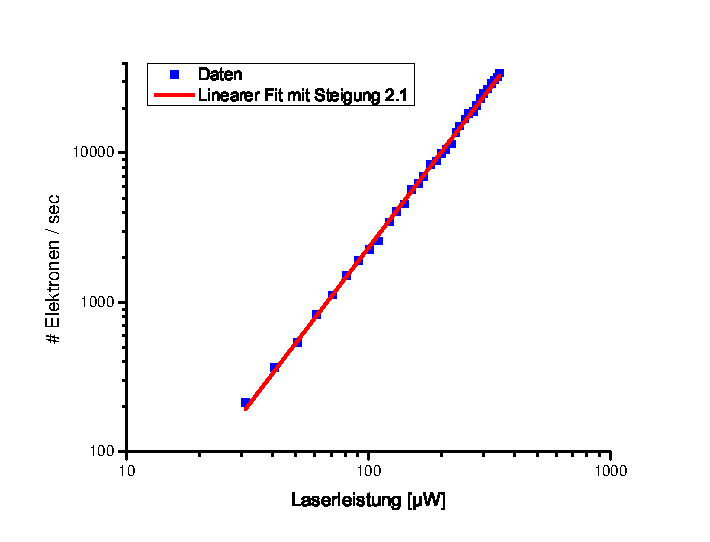
\includegraphics[width=0.49\textwidth]{480e}}
  \hfill
  \subfigure[520nm - Gefittete Steigung ohne die letzten 28 Werte: $2.6\pm0.1$\label{fig:520e}]
  {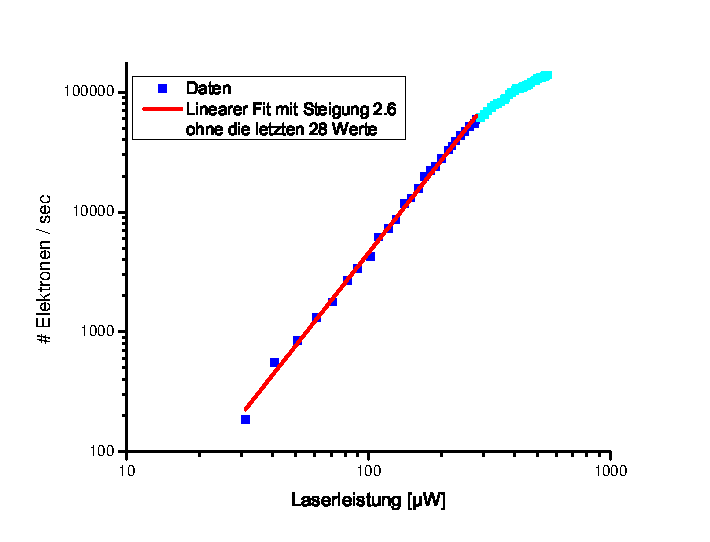
\includegraphics[width=0.49\textwidth]{520e}}
  \hfill
  \subfigure[690nm - Gefittete Steigung: $3.7\pm0.1$\label{fig:690e}]
  {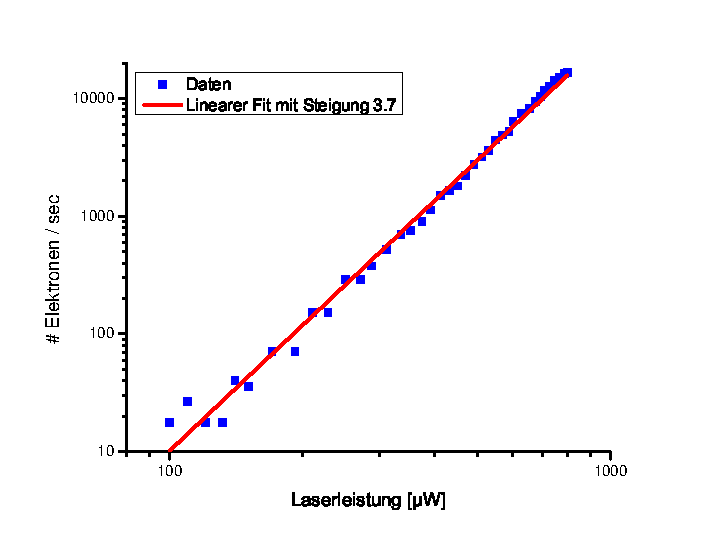
\includegraphics[width=0.49\textwidth]{690e}}
  \caption{Beispielhafte Auftragung des Elektronenstroms gegen die eingestrahlte Intensität zu drei beispielhaften Wellenlängen.}
  \label{fig:e}
\end{figure}


Plottet man wie in Abb. \ref{fig:ges_messung} zu sehen alle Steigungen, so ergibt sich nicht das einfachste zu erwartende Bild einer Treppenfunktion.
Die Gründe hierfür können vielfältig sein: zum Beispiel ist im Gegensatz zu den meisten bisherigen Messungen der Austrittsarbeit wie in Tabelle \ref{tab:austrittsarbeit} nicht eine einzige Kristallebene an der Oberfläche, sondern durch die runde Spitze sind viele verschiedene Facetten an der Oberfläche.
Da jedoch alle Ebenen eine unterschiedliche Austrittsarbeit besitzen, erhält man eine Überlagerung der verschiedenen Austrittsarbeiten, wodurch auch Nichtlinearitäten von 2.5 eine sinnvolle Erklärung bekommen, da die eine Fläche einen 2-Photonen-Prozess, eine andere jedoch einen 3-Photonen-Prozess haben kann.
Dies führt dazu, dass man sowohl energiearme, als auch energiereiche Elektronen detektieren können müsste.
Dies wäre im Rahmen einer zukünftigen Messreihe empfehlenswert zu überprüfen.
Sollte die Hypothese der Überlagerung verschiedener Multiphotonen-Prozesse zutreffen, so kann man bei größeren Wellenlängen keine energetisch schmalbandigen Elektronen zum Beispiel für das Ultrafast Low Energy Electron Defraction (ULEED) Experiment mit dieser Methode bereitstellen.
Dies benötigt sehr energetisch schmalbandige Elektronen, damit die Elektronenpulse durch Dispersion nicht zu stark verlängert werden, was die Zeitauflösung verringern würde<+\cite{uleed}+>.

In Abb. \ref{fig:ges_energie} ist die Nichtlinearität aus Diagramm \ref{fig:ges_messung} multipliziert mit der Photonenenergie der jeweiligen Wellenlänge aufgetragen.
Diese mittlere Energie, die bei einem Emissionsprozess benötigt wird 
Zu erkennen ist, dass bei $\SI{480}{\nano\meter}$ eine Energie von $\SI{5.49}\electronvolt$ vorliegt.
Dies passt gut zu den Literaturwerten.
Dass die Gesamtenergie bei einem Emissionsprozess mit größeren Wellenlängen ansteigt, lässt sich so erklären, dass bei größeren benötigten Photonenanzahlen die Wahrscheinlichkeit, dass ein weiteres zeitgleich ankommt, größer ist.
Mit dieser zusätzlichen Energie ist es dann jedoch möglich, nicht nur Elektronen von der Fermi-Kante, sondern auch aus dem $d$-Band zu emittieren.
Da es von diesen jedoch nach Kapitel \ref{sec:zustandsdichte} um eine Größenordnung mehr Elektronen gibt, steigt die Wahrscheinlichkeit einer Emission.\newline\newline



 



\begin{figure}[h!]
\centering
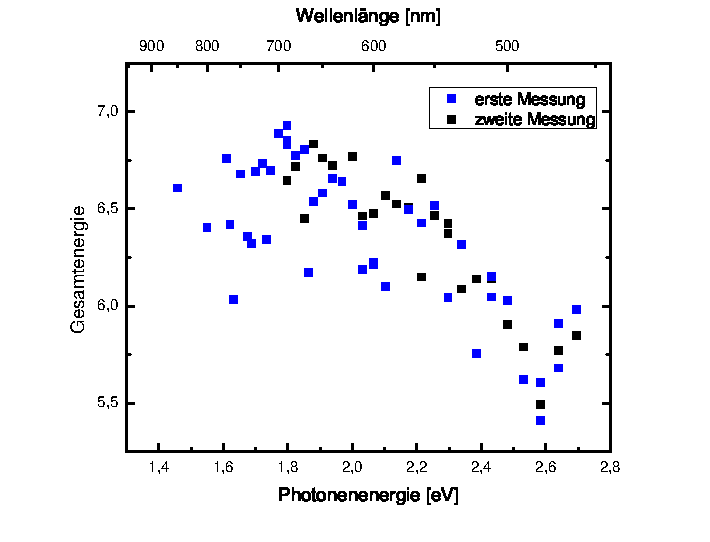
\includegraphics{Gesamtenergie}
\caption{Auftragung der Nichtlinearität aus Abb. \ref{fig:ges_messung} multipliziert mit der jeweiligen Photonenenergie.}
\label{fig:ges_energie}
\end{figure}

In Abb. \ref{fig:ges_messung} ist der Wellenlängenbereich aufgetragen, in dem doppelt gemessen wurde.
Zu erkennen ist, dass die Kurven überwiegend in guter Übereinstimmung liegen und die Ausreißer durch Datenpunkte der jeweils anderen Kurve ausgeglichen werden.
Allerdings ist es nicht auszuschließen, dass manche der Messwerte in blau nicht am Apex, sondern an dem nächsten hellen Spot $\SI{20}{\micro\meter}$ von der Spitze entfernt aufgenommen wurden.
Dies führt dazu, dass manche Werte deutliche Abweichungen von der Kurve zeigen.
Es ist vermutlich nicht darin Begründet, dass die Messungen sehr streuen, da erneute Messungen an den selben Positionen kaum Abweichungen hatten.
\begin{figure}[h]
	\centering
	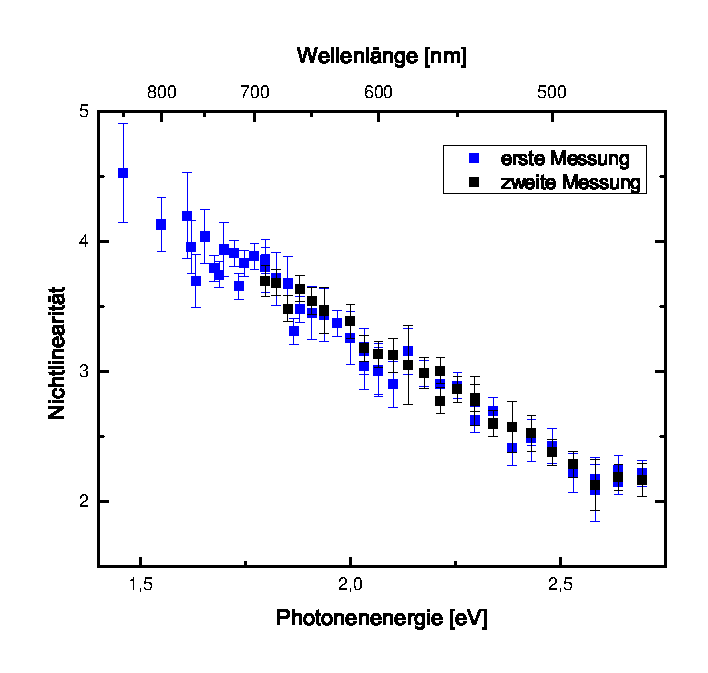
\includegraphics{Vergleich}
	\caption{Vergleich der ersten mit der zweiten Messung der Nichtlinearität in dem doppelt vermessenen Wellenlängenbereich. Zu erkennen ist, dass die beiden Messreihen vergleichbare Ergebnisse lieferten und meist in den Fehlerintervallen der jeweils anderen.}
	\label{fig:ges_messung}
\end{figure}

\begin{figure}[h]
	\centering
	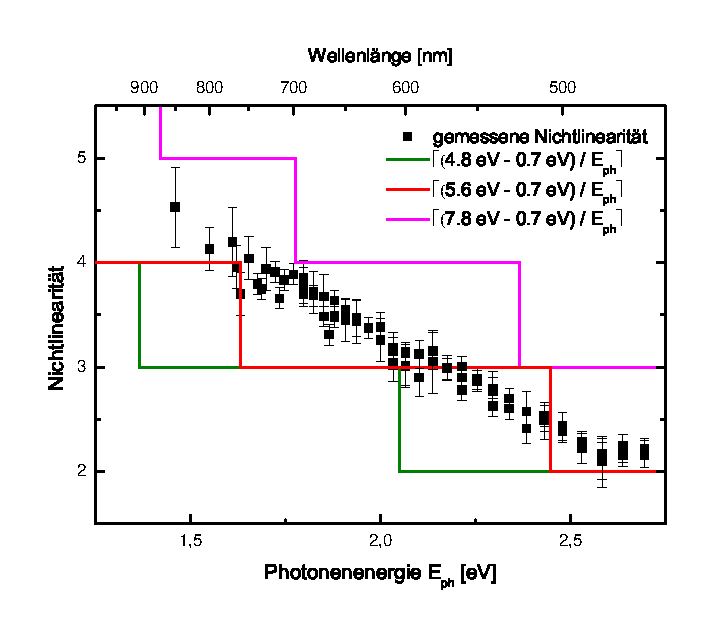
\includegraphics{Stufen}
	\caption{Daten aus Abb. \ref{fig:ges_messung} zusammen mit den einfachst denkbaren Modellen, welche eine Stufen sind. Eingetragen sind in grün mit \SI{4.8}\eV Austrittsarbeit ein niedriger Wert der Fermienergie aus \cite{trasatti_operative_1974}, welcher die Daten nach unten hin begrenzen sollte. In rot ist der höchste Wert einer Austrittsarbeit für eine Facette nach \cite{gold_hoch} eingezeichnet als Referenz, um zu sehen, ob Elektronen ausschließlich von der Fermikante kommen. Wäre dies der Fall, so müssten die Daten zwischen den beiden Kurven liegen. In pink ist dann die ungefähre Lage des $d$-Bandes eingezeichnet. Klar zu erkennen ist, dass die Messwerte zwischen der grünen und der pinken, jedoch auf beiden Seiten der roten Kurve liegen.}
	\label{fig:stufen}
\end{figure}


In Grafik \ref{fig:regenbogen} sind ausgewählte Messreihen zusammen dargestellt.
Erkennbar ist, dass mit steigender Wellenlänge die Geradensteigung zunimmt, der Achsenabschnitt jedoch nicht konstant ist.
Die Farbe der Geraden entspricht in etwa der des Lichtes, bei der die Gerade gefittet wurde.


\begin{figure}[h]
	\centering
	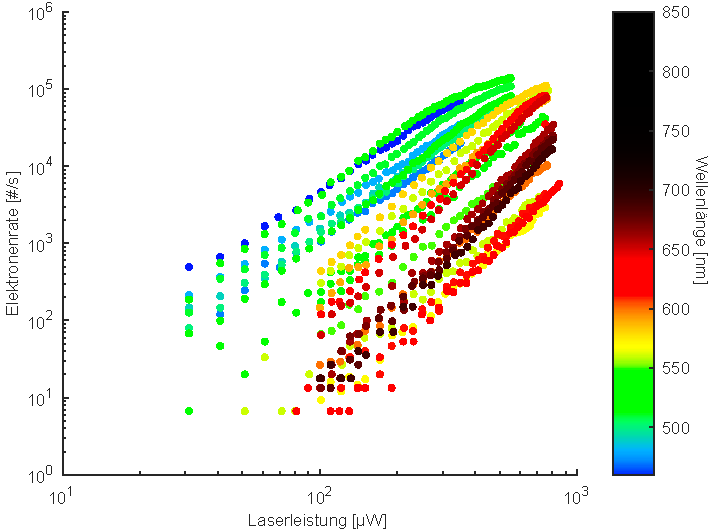
\includegraphics[width=0.7\textwidth]{Faecher_Daten}
	\caption{Ausgewählte Messreihen verschiedener Wellenlängen aufgetragen. Die Farbe der Messpunkte entspricht in etwa der wahrgenommenen Farbe des Lichts.}
	\label{fig:regenbogen}
\end{figure}


% \section{Spannungsscan}
% Der zweite Teil der Messung bestand in einem Spannungsscan.
% Dabei wurde bei konstanter Wellenlänge die Spannung in \SI{20}{\V} Schritten von 500 auf \SI{100}{\V} gesenkt.




\chapter{Diskussion und Ausblick}
In diesem Abschnitt soll auf mögliche Fehlerquellen eingegangen werden, sowie ein Ausblick auf mögliche zukünftige ergänzende Experimente gegeben werden.

\section{Stabilit\"at der Laserintensit\"at}
Die SHG ist sehr sensitiv auf das interne Beampointing, so dass selbst ein relativ geringer Luftzug mit seinen Dichteschwankungen schon deutliche Einbrüche in der Intensität bedeutet.
Dies bedeutet, dass selbst das Vorbeigehen am Laser Einbr\"uche von bis zu 50\% an Leistung bewirkte.
Die Feedback-Schleife war jedoch nicht darauf ausgelegt, kontinuierlich zu regeln, sondern stellte nur zu Beginn jeder Messung die Intensit\"at ein.
W\"ahrend die Bilder aufgenommen wurden regelte sie also nicht nach.
Da jedoch nicht viele Leute an dem Lasersystem vorbeigingen und im sp\"ateren Verlauf der Messungen darauf geachtet wurde, dass w\"ahrend der Messungen kein Luftzug entstand, sind h\"ochstens einzelne Datenpunkte von einzelnen Wellenl\"angen betroffen.


\section{Degradation der Spitze}
In Abb. \ref{fig:rem} sind REM-Aufnahmen der verwendeten Spitze vor und nach dem Experiment gezeigt.
Deutlich zu sehen ist, dass nach den Messungen sich Strukturen auf der Spitze befanden.
Diese Hahnenkamm-ähnlichen Auswüchse haben sehr viel kleinere Radien.
Allerdings ist es möglich, dass sie erst entstanden, als die Spitze aus der Vakuumkammer genommen wurde, um sie ins REM einzubauen.
Bild \ref{fig:spitze_vorher2} ist zwar etwas unscharf, jedoch scheint auch da schon der Krümmungsradius des Apexes gegenüber \ref{fig:spitze_vorher} größer zu sein und eine Ausbuchtung nach oben entstanden zu sein.
Dies ist insofern wahrscheinlich, als dass die Spitze vor dem Ausbau nicht besonders viele Elektronen emittiert hat, wie es bei einer hohen Feldüberhöhung zu erwarten gewesen wäre.
Auch lässt sich ein leichter Farbkontrast zwischen der Spitze und dem gewachsenen erkennen, was dafür spricht, dass es sich bei dem angelagerten Material nicht um Gold handelt.
Denkbar wäre es, dass beim Ausbau durch elektrostatische Felder Schmutz angezogen wurde und sich niedergeschlagen hat.

\begin{figure}[h!]
  \centering
  \subfigure[REM-Bild der Spitze vom 12.06.14\label{fig:spitze_vorher}]
  {\includegraphics[width=0.49\textwidth]{spitze_vorher}}
  \hfill
  \subfigure[REM-Bild der Spitze vom 23.10.14\label{fig:spitze_vorher2}]
  {\includegraphics[width=0.49\textwidth]{spitze_vorher2}}
  \hfill
  \subfigure[REM-Bild der Spitze vom 31.05.16\label{fig:spitze_nachher}]
  {\includegraphics[width=0.49\textwidth]{spitze_nachher}}
  \caption{REM-Bild der Spitze vor und nach den Messungen.}
  \label{fig:rem}
\end{figure}

Als Strahler, der sich ungefähr in der Mitte zwischen Apex und Gitter befand könnten die zwei Körner mit einem Durchmesser von 230 und \SI{260}{\nm} fungiert haben.




\section{Stufen $\Rightarrow$ Gerade}
\begin{itemize}
\item Thermisches Heizen $\Rightarrow$ höherenergetische Elektronen
\item Absorption von niederenergetischeren Elektronen
\item $d$-Band
\item Schottky-Reduktion / heiße Elektronen tunneln
\item Facetten mit unterschiedlicher Austrittsarbeit
\end{itemize}



\section{Die Elektronische Zustandsdichte}
\label{sec:zustandsdichte}

Elektronen mit Spin $\nicefrac{1}{2}$ müssen dem Pauli-Prinzip genügen, nach dem sich keine zwei Elektronen in dem selben Zustand befinden können.
Dies führt dazu, dass mit dem hinzufügen von weiteren Elektronen zu einem System immer energetisch höhere Zustände besetzt werden müssen.
Mit einem Band werden viele energetisch dicht beieinander liegende mögliche Zustände bezeichnet.
In einem Isolator sind alle Bänder entweder komplett gefüllt, oder leer, was dazu führt, dass kein Strom fließen kann.
Auch sind die Bänder im Gegensatz zu einem Halbleiter so weit entfernt, dass keine Elektronen aus einem gefüllten Valenzband (zum Beispiel durch thermische Fluktuation) in ein leeres Band (Leitungsband) kommt.
Ist dies der Fall, so können sowohl Elektron, als auch Loch zu einem Stromfluss beitragen.
Bei Metallen ist mindestens eines der Bänder nur teilweise gefüllt, wodurch ein Strom fließen kann.

Durch die Interaktion zwischen Kristallgitter mit dem periodischen Potential und den Elektronen ergibt sich die sogenannte elektronische Zustandsdichte.
Mit der elektronischen Zustandsdichte werden die Anzahl von stationären Elektronenzuständen in einem Energieintervall und Volumen bezeichnet.

In Abb. \ref{fig:gold_zustandsdichte} ist diese für Gold aufgeführt.
Zu sehen ist, dass es um eine Größenordnung mehr Elektronen gibt, die im $d$-Band $\SI2{\electronvolt}$ weniger Energie besitzen, als die Fermi-Energie.
Dies bedeutet, dass zur Ionisierung zwar ungefähr ein Photon mehr benötigt wird, es jedoch auch deutlich mehr Elektronen gibt.

Aufgrund der Tatsache, dass ein drei-Photonen-Prozess bei gleicher Intensität deutlich unwahrscheinlicher ist, als ein zwei-Photonen-Prozess, dieser Unterschied jedoch nicht so stark bei höheren Ordnungen ist, ist zu erwarten, dass je höher die Nichtlinearität ist, mehr Elektronen aus dem $d$-Band gelöst werden.

\begin{figure}[h!]
	\centering
	\includegraphics{GoldZustandsdichte}
	\caption{Elektronische Zustandsdichte aus \cite{gold_zustandsdichte}}
	\label{fig:gold_zustandsdichte}
\end{figure}






%\chapter{Zusammenfassung}


\appendix
\chapter{Anhang}
\begin{figure}[h]
	\centering
	\includegraphics[width=0.7\linewidth]{Orpheus_Tuning_Curve}
	\caption{Ausgangsleistung des Orpheus im gesamten emittierenden Wellenlängenbereich aus dem Datenblatt des Herstellers \cite{orpheus_tuningcurve}.}
	\label{fig:orpheus_tuningcurve}
\end{figure}


\cleardoublepage
%% Bibliographie. Das Argument muss der Name der BIBTeX-Datenbank stehen.
%% Ein Beispiel fuer eine solche Datenbank finden Sie in bthesis_datenbank.bib
\bibliography{bthesis_datenbank}

\begin{comment}
\chapter*{Danksagung}
Mein Dank geht in erster Linie an Claus Ropers, der mir die Möglichkeit gab, diese äußerst spannende Arbeit durchzuführen und der mir mit fachlichen Anregungen stets zur Seite stand.\\

Ebenfalls möchte ich Dr. Reiner Bormann und Benjamin Schröder für die ausgezeichnete Betreuung danken.
Auch Gerrit Horstmann unterstützte mich stets (nicht nur moralisch mit Eis!).\\

Bei Herrn Prof. Jooß möchte ich mich für die freundliche Bereitschaft bedanken, die Zweitkorrektur zu übernehmen.\\

Der Arbeitsgruppe möchte ich für die ausgesprochen angenehme Athmosphäre sowohl im wissenschaftlichen, als auch im sozialen danken.\\




Ebenfalls Dank gebührt Nicolas Wöhrl und Reinhard Remfort vom Podcast \textit{Methodisch Inkorrekt}, da sie mir mit ihren interessanten wissenschaftlichen Themen zahlreiche Stunden im Labor angenehm gemacht haben.\\\\

Natürlich möchte ich mich nicht zuletzt bei meiner Familie bedanken, dass sie es mir ermöglichen, ein so interessantes Studium zu ermöglichen und mich stets unterstützten.
\end{comment}


%% Dieser Befehl MUSS am Ende stehen und erzeugt die Erklaerung ueber die
%% benutzten Mittel
\Declaration
\end{document}
